\chapter{Background} \label{chapter:BACKGROUND}

This chapter describes prototype-based programming, the Lively Kernel, and CoExist.
These works are the background of this thesis as we introduce an approach for providing CoExist-like recovery support in prototype-based programming systems, which we implemented for the Lively Kernel.

\section{Prototype-based Programming}

Prototype-based programming is object-oriented programming in which applications are created directly with objects, without requiring developers to define classes first.\\
Self, JavaScript, and Kevo~\cite{Taivalsaari1992Kevo} are prototype-based programming languages.
Many end-user programming systems such as Scratch~\cite{Maloney2010SPL}, Etoys~\cite{Kay2005Etoys}, and Fabrik~\cite{Ingalls1988FVP} also enable users to express programs using objects.

Prototype-based programming allows to build applications from particular objects.
This is the fundamental difference to the class-based style of object-oriented programming, in which programs are expressed with classes.
Each part of a prototype-based program has particular state.

There are different advantages associated with this kind of programming:
\begin{itemize}
    \item \cite{Taivalsaari1996CVP} and \cite{Lieberman1986UPO} suggest that it might be easier for programmers to understand concrete examples than to grasp abstract classes. A concrete example provides particular values for its state and, in case of objects with a visual appearance, can be actually looked at.
    \item \cite{Ungar1987SPS} and \cite{Borning1986CVP} describe how prototype-based programming makes it easier to introduce one-of-a-kind objects with their own structure or behavior.
    \item \cite{Borning1986CVP} and \cite{Maloney1995Mor} argue that especially editing visual objects can be more concrete with prototypes. Instead of writing code that describes the appearance of objects, programmers can manipulate visual objects directly. Programmers could, for example, use the mouse to manipulate properties like the size, position, or to combine multiple elements. This way, programmers always see intermediate states instead of only receiving feedback on explicit test runs in-between edit-compile-load cycles. 
\end{itemize}

\paragraph{Editing Graphical Objects at Runtime}
Many prototype-based programming systems, including the examples given in this section, allow to manipulate objects at runtime.
Scratch, Etoys, Fabrik, the Lively kernel, and Self all provide tools dedicated to manipulating graphical objects directly.
Such graphical objects range from basic objects like primitive shapes to complete applications like presentation software or programming tools.
Prototype-based programming, programming at runtime, and direct manipulation of graphical objects seem to be properties that suit each other.

\paragraph{Similar Objects Without Classes}
Different prototype-based programming systems provide different approaches for creating similar objects.
Self and JavaScript incorporate \emph{delegation} to allow for prototypical inheritance.
Objects can inherit state and behavior directly from other objects: each object has a \emph{prototype} to which it delegates whenever looking up a property in the object itself yields no results.
In Self, the prototype of an object is set when objects are cloned: The clone's prototype is the object it was cloned from.\\
In JavaScript, objects are created from constructor functions.
The constructor function's prototype becomes the prototype of created objects.\\
Kevo, in constrast, does not incorporate this notion of prototypical inheritance.
It provides \emph{concatenation} for incremental modification of objects~\cite{Taivalsaari1995DVC}.
Objects are copied to create objects with the same state and behavior as existing objects.
These objects are self-contained.
Changing an object only changes that particular object and a particular object can only be changed by directly changing it, not by changing any other object.
To adapt many objects at once, programmers can use so-called \emph{module operations} in Kevo.
Module operations are evaluated for groups of objects.


\section{The Lively Kernel}

The Lively Kernel is a programming system in the tradition of Smalltalk and Self.
Development happens at runtime.
It incorporates tools and techniques to be completely self-sufficient.
Thus, programmers can create versions of the Lively Kernel with the Lively Kernel.

The Lively Kernel is a browser-based system.
It is implemented in JavaScript and renders to \ac{html}.

\subsubsection{Programming with Prototypes and Classes}

As the Lively Kernel is based in JavaScript, the system and applications are expressed in a prototype-based object-oriented language that provides prototypical inheritance.
At the same time, the Lively Kernel also provides a class system and considerable parts of the system are expressed using classes.

The Lively Kernel implements Morphic~\cite{Maloney1995Mor}, a framework for developing graphical applications.
The graphical objects of this framework are called \emph{Morphs}.
Each morph has a class but can also have object-specific behavior.
They can be created by instantiating a class or by copying an existing morph.
Morphs are often edited directly and not through adapting existing or creating new classes.
This way, the Lively Kernel mixes the class-based with the prototype-based style of object-oriented programming.

The Lively Kernel's copy operation does not establish a prototypical inheritance relationship between the copy and the original.
Instead, it creates a full copy of the original morph's properties, including its class.
Therefore, even though JavaScript incorporates prototypical inheritance, the Lively Kernel encourages programmers to use classes to share behavior among objects.

\subsubsection{Direct Manipulation of Morphs}

Programmers can change the position of morphs by \emph{dragging} and the composition by an alternative dragging, called \emph{grabbing}.
When a morph is grabbed, it can be added to another morph and becomes that morph's submorph.
This way, a morph does not have to be a basic shapes or simple widgets, but can be the interface of any application.

\begin{figure}[h]
    \centering
    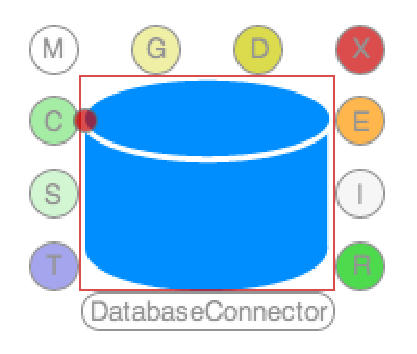
\includegraphics[width=0.3\textwidth]{figures/2_background/1_halos.pdf}
    \caption{The halo buttons of a basic morph.}
    \label{fig:Halos}
\end{figure}

The Lively Kernel provides a set of manipulation tools, called \emph{Halos}, as shown in Figure~\ref{fig:Halos}.
Developers can bring up these tools for each morph.
The different buttons of a morph's halo allow, for example, to resize, rotate, and copy morphs.

Other halo buttons open specific tools, which are shown in Figure~\ref{fig:LivelyTools}:

\begin{enumerate}
    \item The \emph{Inspector}~\circnum{1} presents all the values that make up a morph's current state. It also has a small code pane at the bottom that can be used to manipulate the morph's properties programmatically.
    \item The \emph{Style Editor}~\circnum{2} allows to manipulate certain aspects of a morph's visual appearance. Programmers can use it to change, for example, a morph's color, border width, or the layout of its submorphs.
    \item The \emph{Object Editor}~\circnum{3} is a tool to edit the object-specific behavior of morphs. It shows all scripts of a particular morph and allows programmers to add, remove, and edit scripts.
\end{enumerate}

\begin{figure}[h]
    \centering
    \includegraphics[width=\textwidth]{figures/2_background/2_LivelyTools.pdf}
    \caption{Three Lively Kernel's tools to manipulate morphs: the Inspector, the Style Editor, and the Object Editor.}
    \label{fig:LivelyTools}
\end{figure}

\subsubsection{Saving Morphs to the Shared Parts Bin Repository}

A related tool is the Lively Kernel's \emph{Parts Bin}~\cite{Lincke2012LPC}, an object repository to commit and load specific versions of morphs.
Morphs saved to the Parts Bin are called \emph{parts} to emphasize the ability to reuse any of the morphs in the Parts Bin for other morphic applications.
Figure~\ref{fig:PartsBin} shows the Parts Bin, opened on the \emph{Tools} category, which includes both the Style Editor and the Object Editor.
Both these tools are examples for graphical applications developed from available parts.
Their functionality is expressed in scripts and they are available to users through the Parts Bin.

\begin{figure}[h]
    \centering
    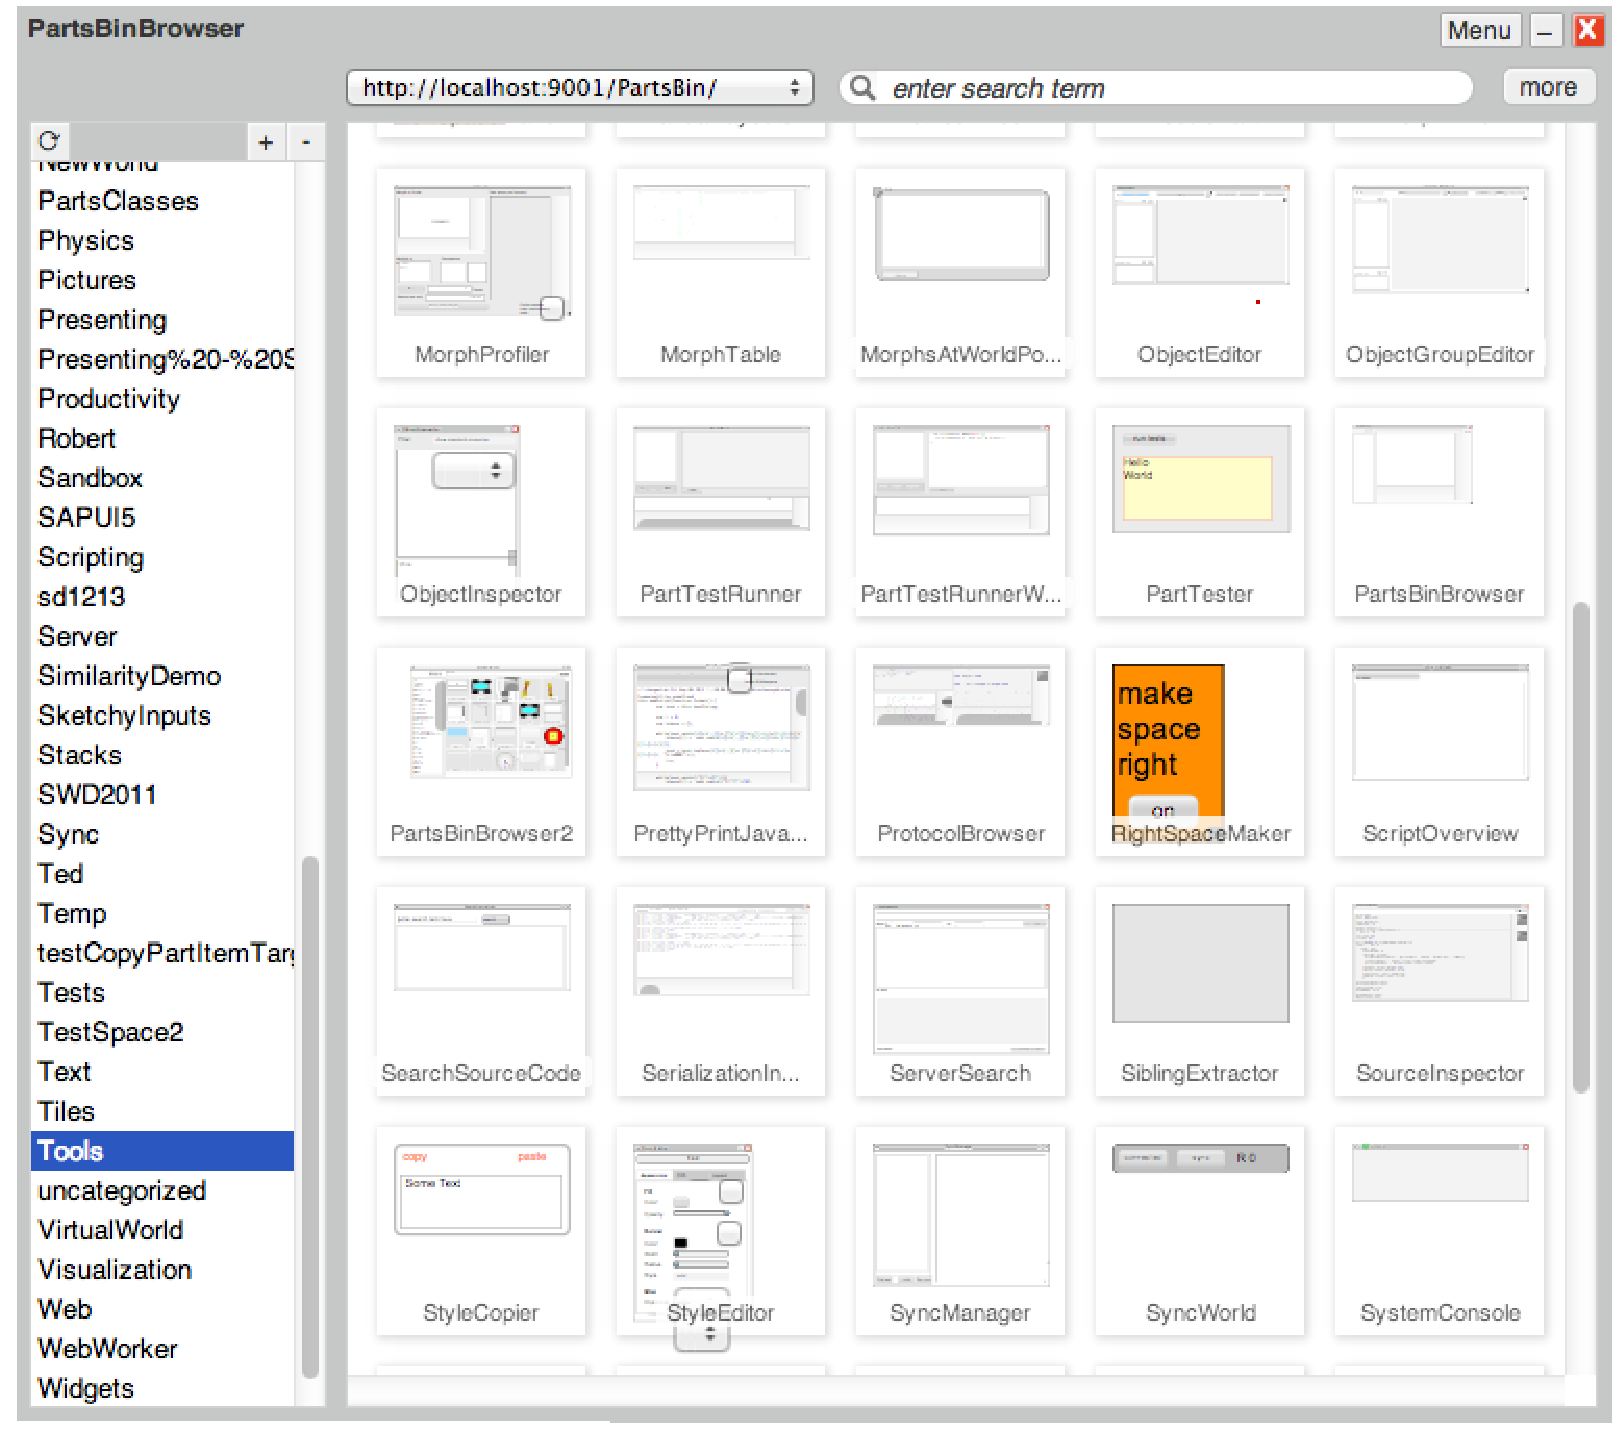
\includegraphics[width=0.7\textwidth]{figures/2_background/3_partsBin.pdf}
    \caption{The Lively Kernel's Parts Bin opened on the \emph{Tools} category.}
    \label{fig:PartsBin}
\end{figure}

The root of the scenegraph of visible morphs is called \emph{World}.
Worlds are not shared via the Parts Bin, but can be saved as a Web pages.
A world stores the state of all visible morphs when saved and that state can be reloaded with the world.


\section{CoExist}

CoExist\footnote{\url{http://www.bastiansteinert.org/coexist.html}, accessed February 28, 2014} provides recovery support to programmers.
It continuously preserves access to intermediate development state.
The states are recorded as separate version in their original order. 
For each version CoExist provides access to diffs, test results, and screenshots of the development environment.
Programmers can review their programming sessions, inspect the impact changes had on test cases, and recover information from previous development states.

\subsubsection{Tools to Recover Previous Development States}

CoExist provides two tools to help programmers benefit from the preserved histories, shown in Figure~\ref{fig:CoExist}.

\paragraph{Timeline}
CoExist's \emph{Timeline} tool is located at the bottom of the development environment.
It shows each intermediate version with a small rectangle.
The color of the rectangle's four corners indicate test results: the bottom of the rectangle shows how many test cases passed and failed absolutely, while the top highlights how the changes of a version affect test results.\\
Hovering over a rectangle shows which artifact was changed in the version.\\
The versions presented in the timeline can also be re-established.

\paragraph{Version Browser}
Besides the timeline of versions, a \emph{Version Browser} tool provides an overview of the versions.
For each package it shows the changes made in that package.
It presents the same information on test cases, but also includes a diff view.
Moreover, it provides a screenshot of the development environment for each version.

The tools support programmers in re-tracing their steps, understanding the impact of their actions, and in recovering previous development states.
They can withdraw changes permanently or recover only specific information from previous versions.

\begin{figure}[h]
    \centering
    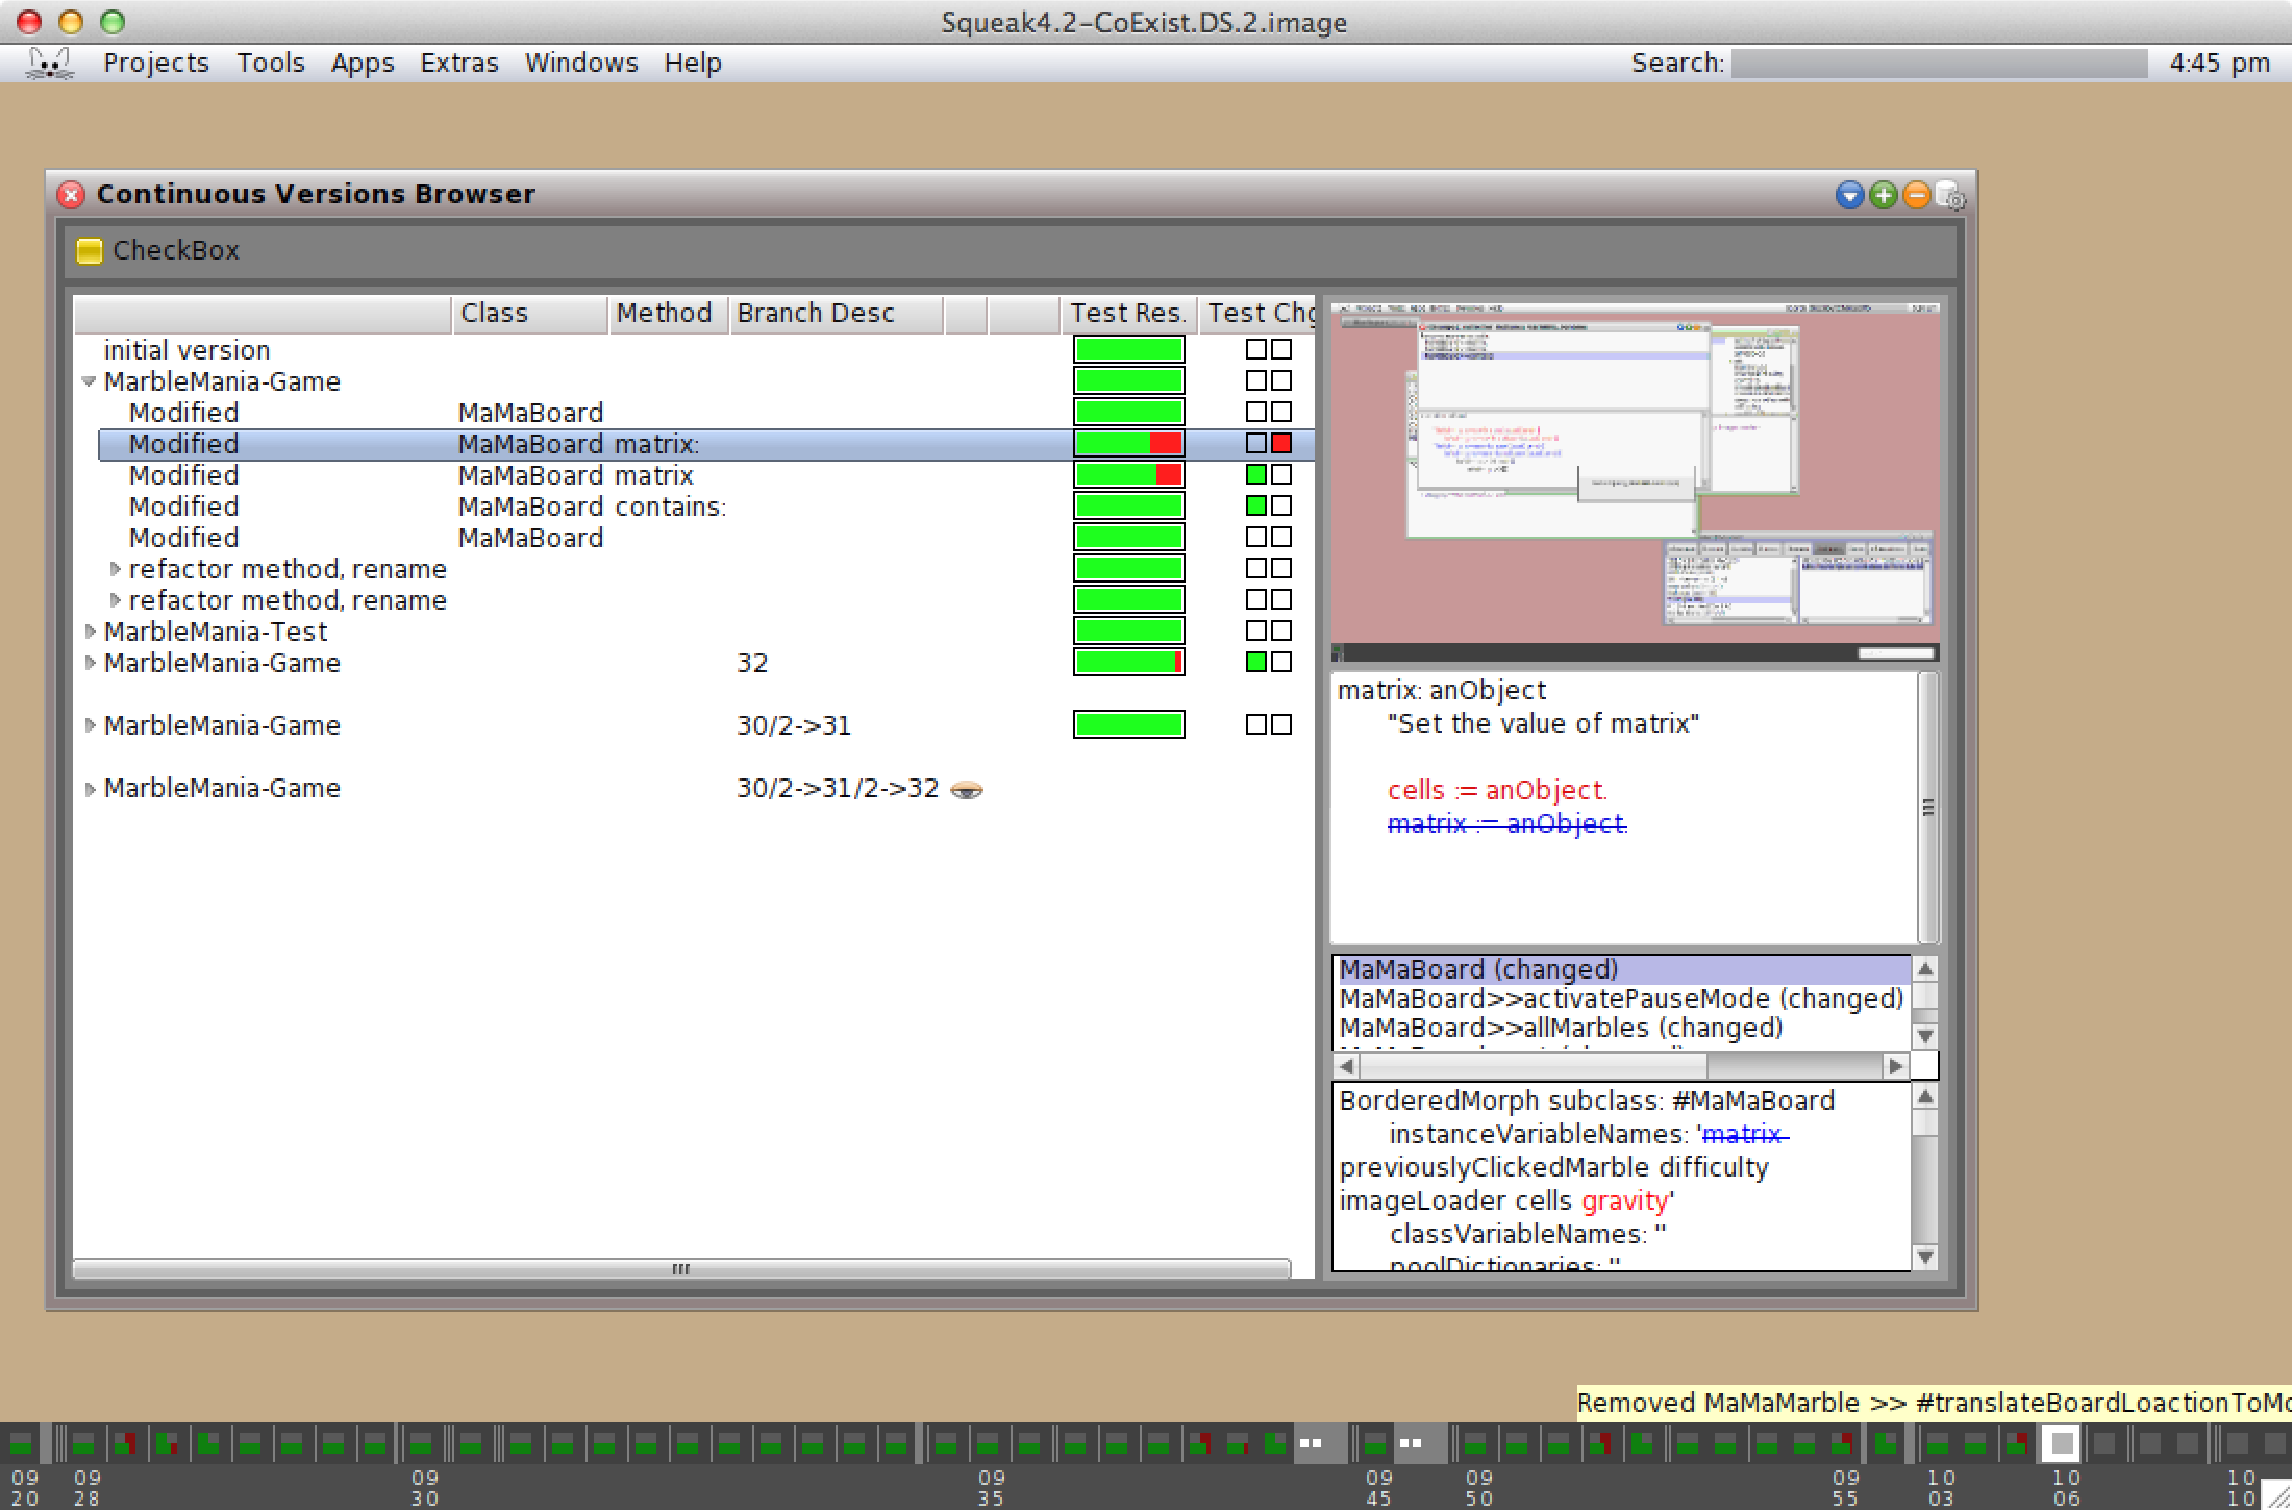
\includegraphics[width=\textwidth]{figures/2_background/4_coexistTools.pdf}
    \caption{CoExist's tools to manage the preserved development states: the \emph{Timeline} and the \emph{Version Browser}.}
    \label{fig:CoExist}
\end{figure}

\subsubsection{Benefits of Continuous Versioning}

CoExist aims at reducing the effort required to recover previous states and, thereby, at encouraging programmers to explore their ideas through making changes to the code.

Without CoExist, either compensational or precautionary actions are necessary for recovery.
When programmers unintentionally introduce errors, decrease performance, or harm the program design, they have to repair changed code.
They either need to edit the code again or load a previously commited version of the code.
Editing code of potentially many methods across and many classes is obviously a significant effort and error-prone.
Loading a previous version is only possible if a version has been commited previously.
Therefore, programmers can reduce the cost of recovery by anticipating recovery needs beforehand.
However, preserving versions is also an effort and especially so when revision histories are expected to be well-documented and immediately useful.
For that, programmers need to assemble changes to meaningful increments, run tests, and write helpful commit messages.

CoExist, in contrast, makes recovery fast and easy.
It is similar to the undo/redo of applications.
Developers do not have to take explicit precautionary actions, but are still able to undo changes when necessary.
However, CoExist provides convenient access to the previous states of entire systems not just to a particular source code view.
It presents the preserved versions with additional information.
Each version is associated with the static structure of the software system, related to other versions in a timeline, and accompanied by test results.
Furthermore, making changes to a previous state in CoExist does not overwrite the history, but creates a branch.

\emph{In essence}, instead of worrying about negative consequences, programmers can focus on implementing their ideas and rely on CoExist to help in case any action unexpectedly needs to be undone.
